\apendice{Documentación técnica de programación}

\section{Introducción}

\section{Estructura de directorios}

...

\begin{figure}[h]
	\caption[Diagrama: estructura de directorios]{Diagrama que representa la estructura física de directorios en el repositorio.}
	\centering
	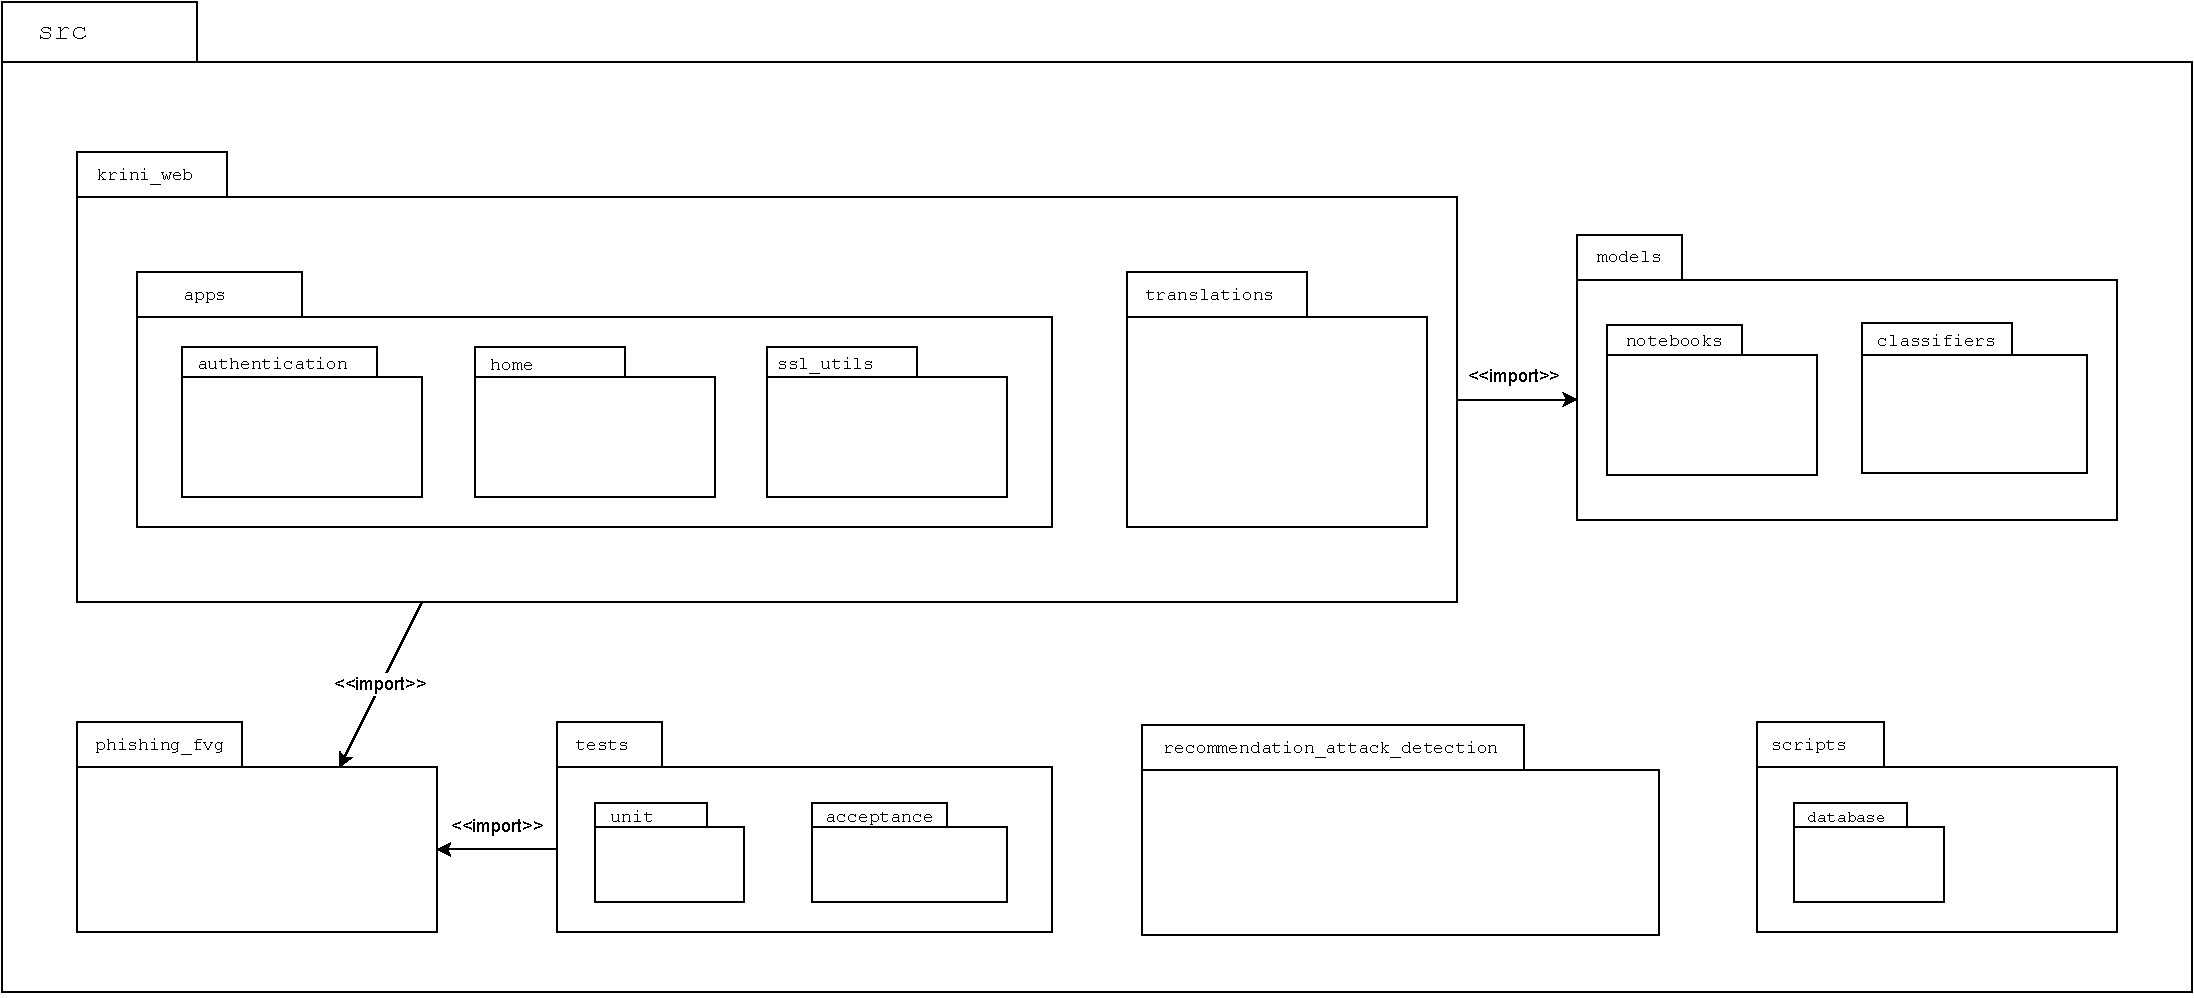
\includegraphics[width=\textwidth]{../img/anexos/diagrams/repo-structure}
	\label{d:diag-repo-structure}
\end{figure}

\section{Manual del programador}

\section{Compilación, instalación y ejecución del proyecto}

\section{Compilación, instalación y ejecución de herramientas auxiliares}

\begin{figure}[h]
	\caption[\textit{Co-forest}: Configuración de un experimento en KEEL]{Configuración de un experimento que utiliza el algoritmo \textit{co-forest} mediante la GUI de KEEL.}
	\centering
	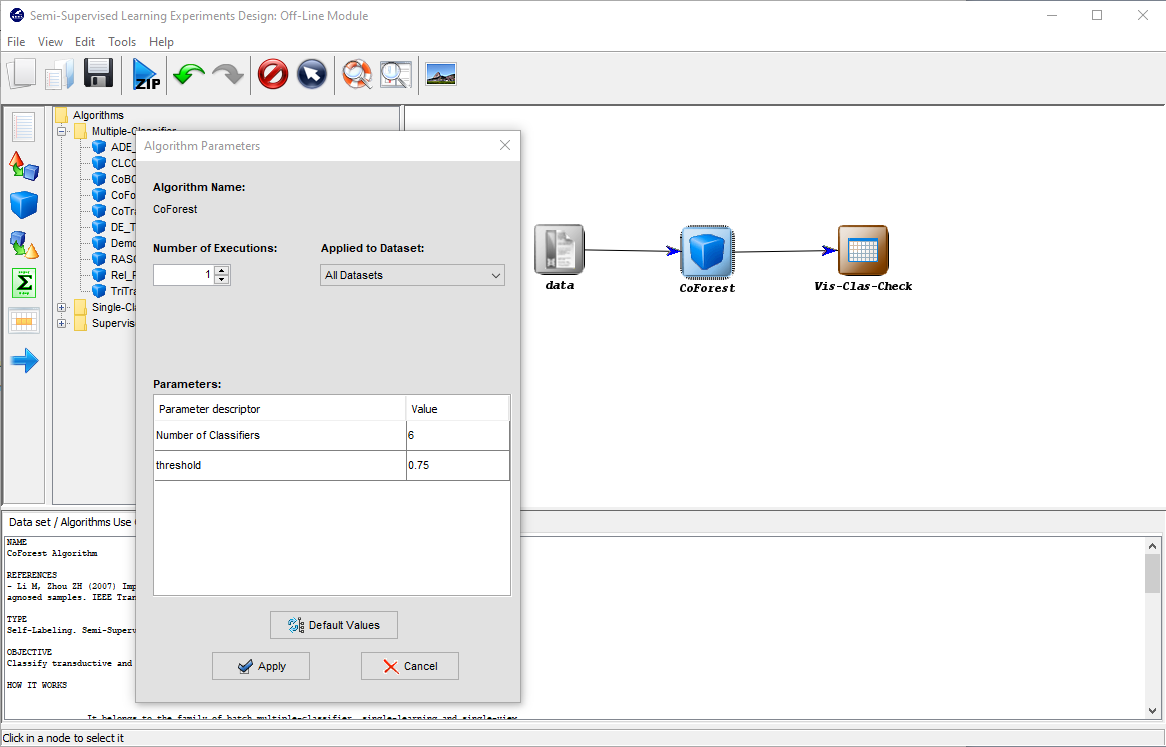
\includegraphics[scale=0.5]{../img/anexos/manual/keel_gui.png}
\end{figure}

\subsection{KEEL}

KEEL es una herramienta que permite experimentar con modelos de \textit{machine learning}. Ha sido creada por distintas universidades españolas y financiada por el Ministerio de Educación y Ciencia~\cite{KEEL}.

Para poder ejecutarla, en primer lugar, se han de descargar los ficheros fuente del repositorio de GitHub~\cite{keelRepo}. Una vez se han descargado, se compilan aprovechando el fichero \texttt{build.xmlz} contenido y la herramienta \texttt{ant}. Mediante el comando \texttt{ant cleanAll} se eliminan barios previos (para evitar conflictos), y mediante el comando \texttt{ant} se compila el código fuente.

Posteriormente se ejecuta la aplicación mediante el comando \texttt{java -jar ./dist/GraphInterKeel.jar} y se utiliza mediante su interfaz gráfica.


\section{Pruebas del sistema}
\label{s:pruebas}

Las pruebas \textit{software} son un proceso sistemático y controlado para evaluar y verificar el correcto funcionamiento de un producto. Están reguladas por la ISO/IEC/IEEE 29119~\cite{iso-pruebas} y son fundamentales ya que permiten detectar errores y defectos antes del despliegue, pudiendo así ahorrar costos, tiempo, y facilitando la satisfacción del cliente.

Existen distintos tipos de pruebas en función de qué se está evaluando. Generalmente se sigue un enfoque de más bajo nivel a más alto nivel, iniciando en las pruebas unitarias y finalizando en las pruebas de aceptación.


\subsection{Pruebas unitarias}
\label{s:pruebas-unitarias}

Las pruebas unitarias se centran en comprobar el correcto funcionamiento de las partes individuales del \textit{software}. Se llevan a cabo a nivel de código y están diseñadas para detectar errores y defectos en unidades de menor tamaño (por ejemplo funciones o clases).

Debido a que los algoritmos de ML cuentan con pruebas independientes (comparaciones con otras implementaciones) y la \textit{web} cuenta con las pruebas descritas en la sección~\ref{s:pruebas-aceptación}, se han realizado pruebas unitarias para la clase de utilidades \texttt{phishing\_utils}.

Además, las pruebas unitarias se han automatizado mediante Travis CI, de forma que cada vez que se hace un \textit{push} a las ramas principales o de desarrollo se dispara una \textit{build} que las ejecuta automáticamente como se muestra en la imagen~\ref{d:cp-travis}.

\begin{figure}[h]
	\caption[TravisCI: ejecución automática de pruebas unitarias]{Ejecución automática de las pruebas unitarias mediante TravisCI.}
	\centering
	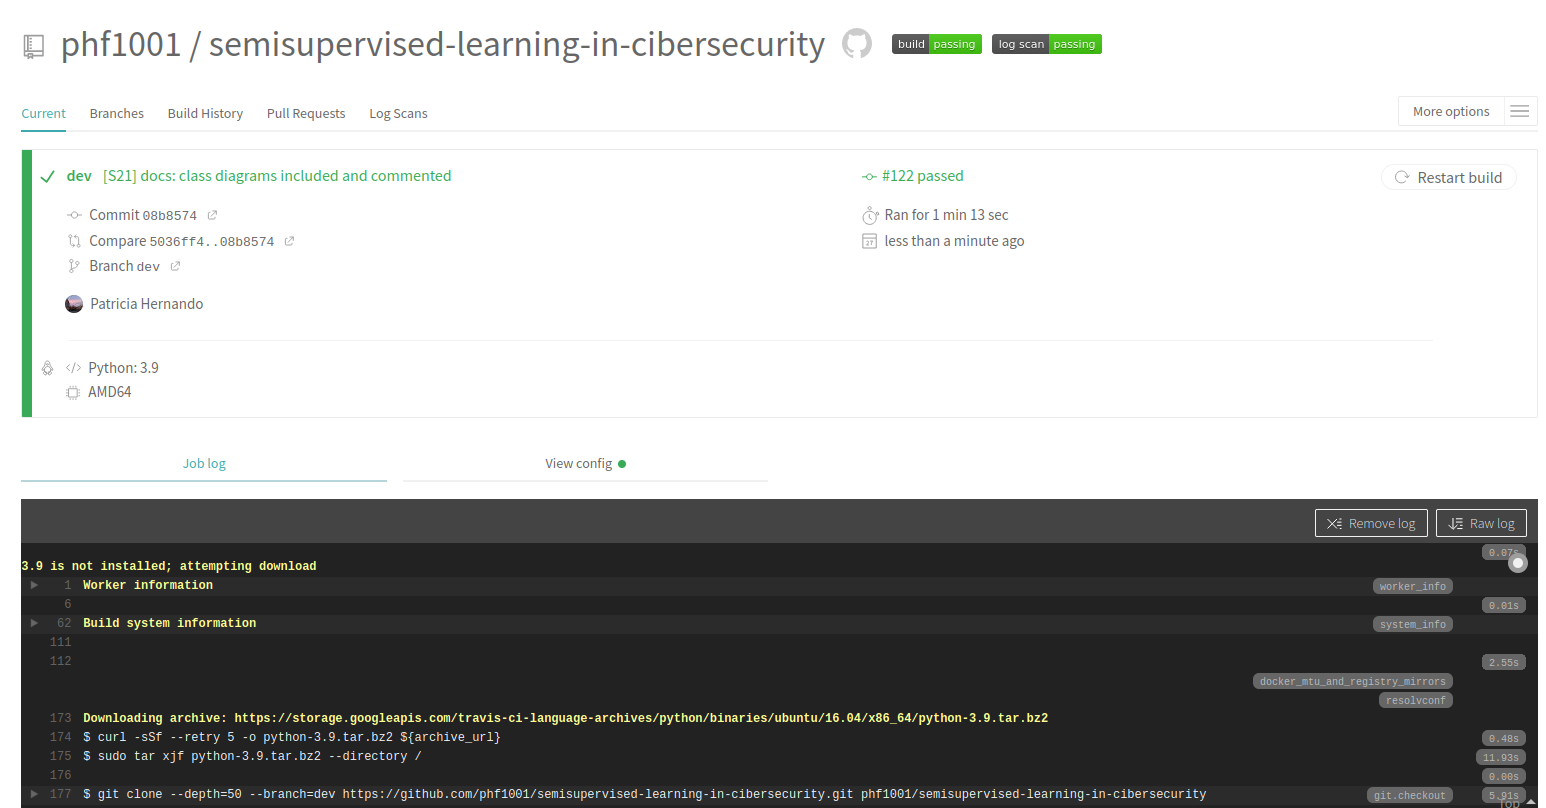
\includegraphics[width=\textwidth]{../img/anexos/cp/travis-tests}
	\label{d:cp-travis}
\end{figure}


\subsection{Pruebas de aceptación}
\label{s:pruebas-aceptación}

Las pruebas de aceptación se realizan para verificar si el \textit{software} está listo para su implementación y si cumple con los criterios de aceptación del cliente. En este proyecto se han querido evaluar algunos de los casos más <<extraños>> con el fin de comprobar su correcto funcionamiento. Estos se han organizado en tres \textit{test suites} divididas por categorías.

Todos los casos de prueba mostrados en las tablas han sido automatizados utilizando Selenium (como se puede observar en la imagen~\ref{cp:selenium}). Los \textit{tests} se facilitan en el repositorio de la aplicación, además de los datos necesarios para ejecutarlos.

\begin{figure}[h]
	\caption[Selenium: ejecución automática de pruebas de aceptación]{Ejecución automática de las pruebas de aceptación y seguridad con la herramienta Selenium.}
	\centering
	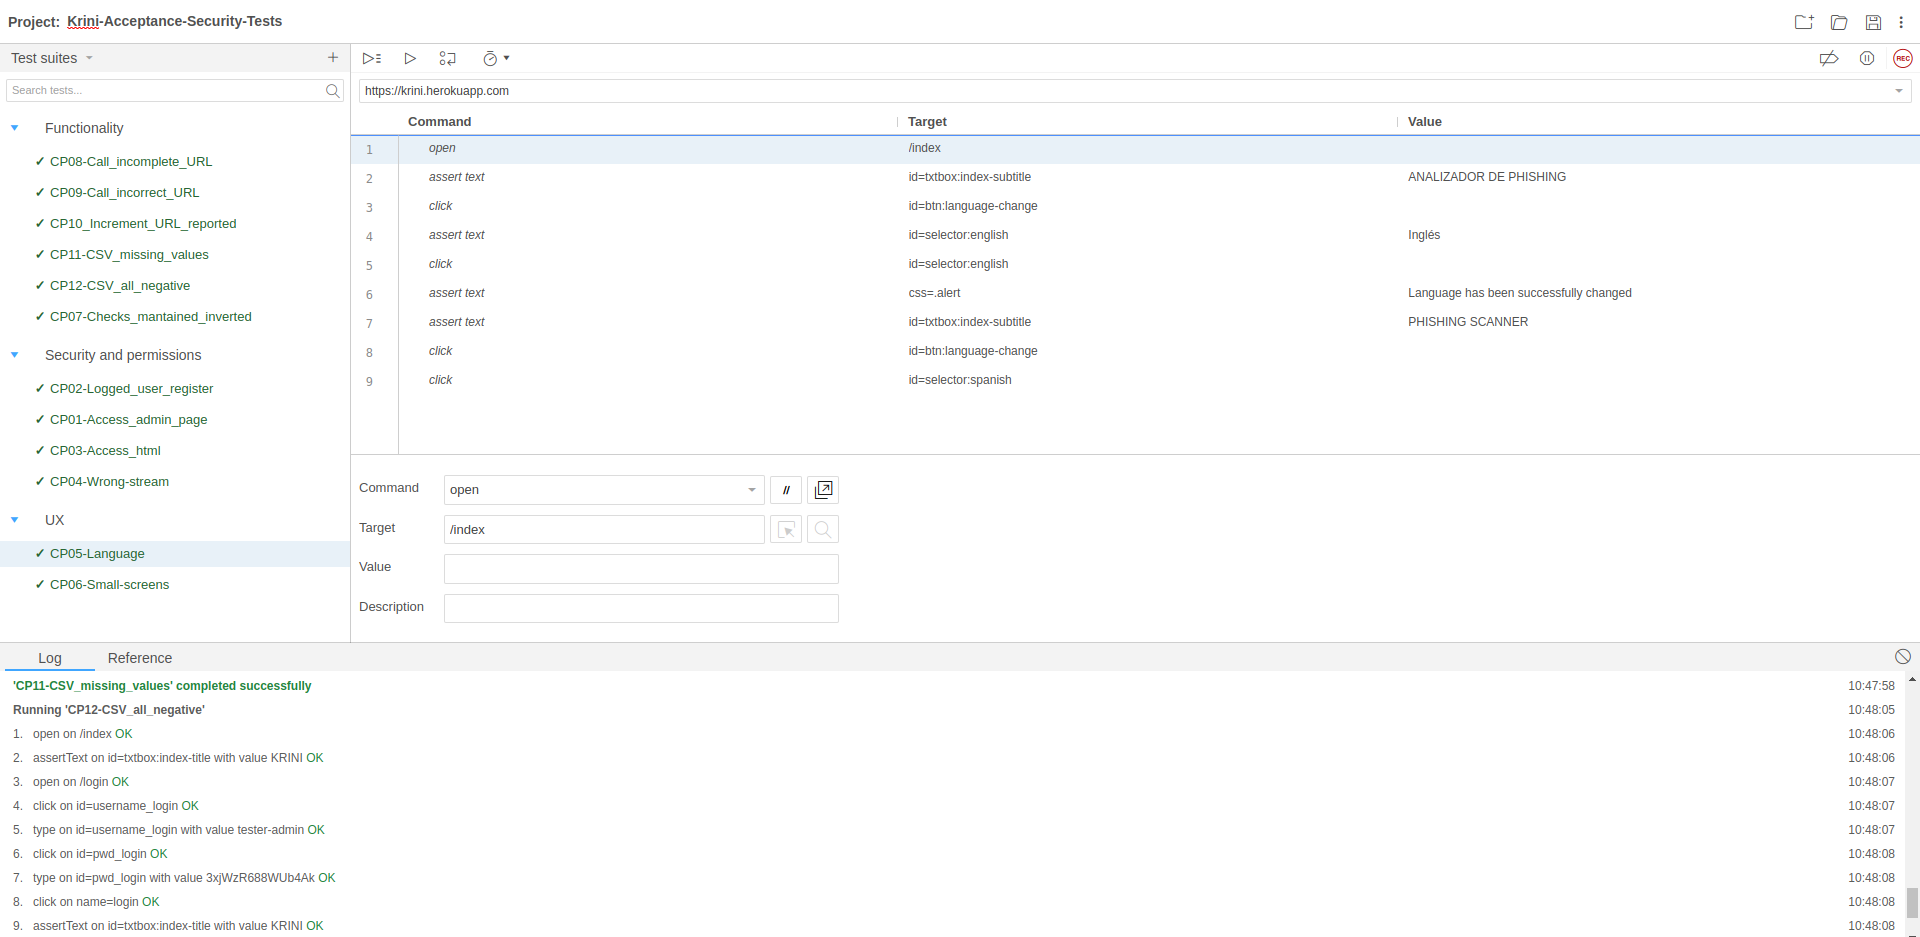
\includegraphics[width=\textwidth]{../img/anexos/cp/selenium-tests}
	\label{cp:selenium}
\end{figure}

\begin{table}[p]
	\centering
	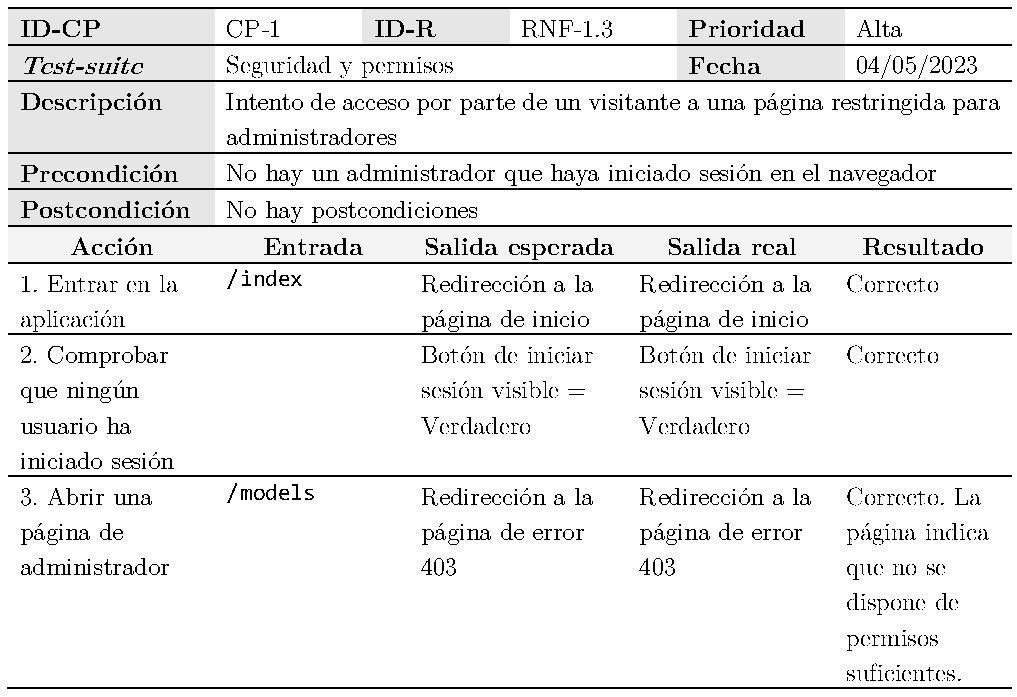
\includegraphics[width=\textwidth]{../img/anexos/cp/CP-1}
	\caption{CP-1 Acceso a página restringida.}
	\label{cp:acc-restringido}
\end{table}

\begin{table}[p]
	\centering
	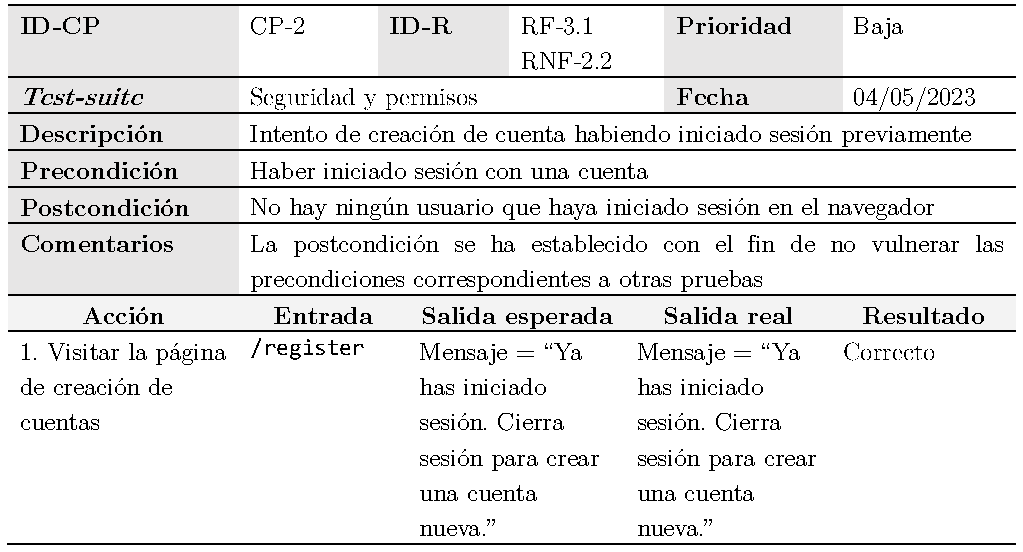
\includegraphics[width=\textwidth]{../img/anexos/cp/CP-2}
	\caption{CP-2 Intento de registro con cuenta accedida.}
	\label{cp:registro}
\end{table}

\begin{table}[p]
	\centering
	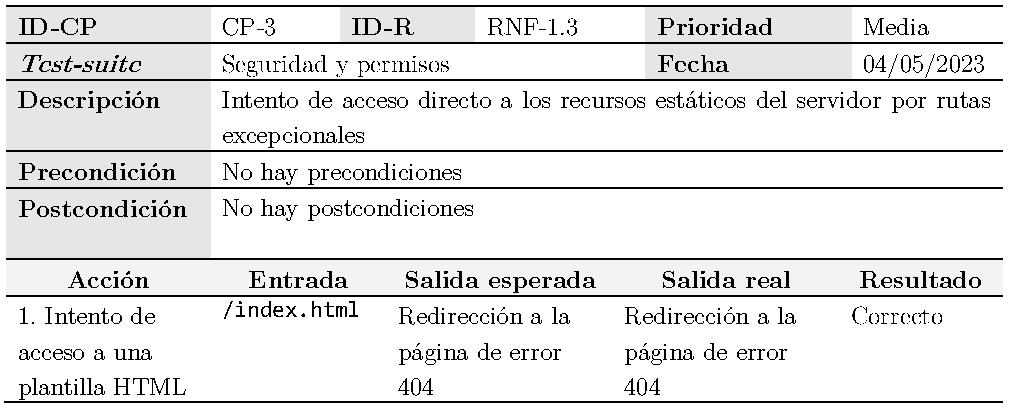
\includegraphics[width=\textwidth]{../img/anexos/cp/CP-3}
	\caption{CP-3 Acceso a recursos estáticos.}
	\label{cp:acc-html}
\end{table}

\begin{table}[p]
	\centering
	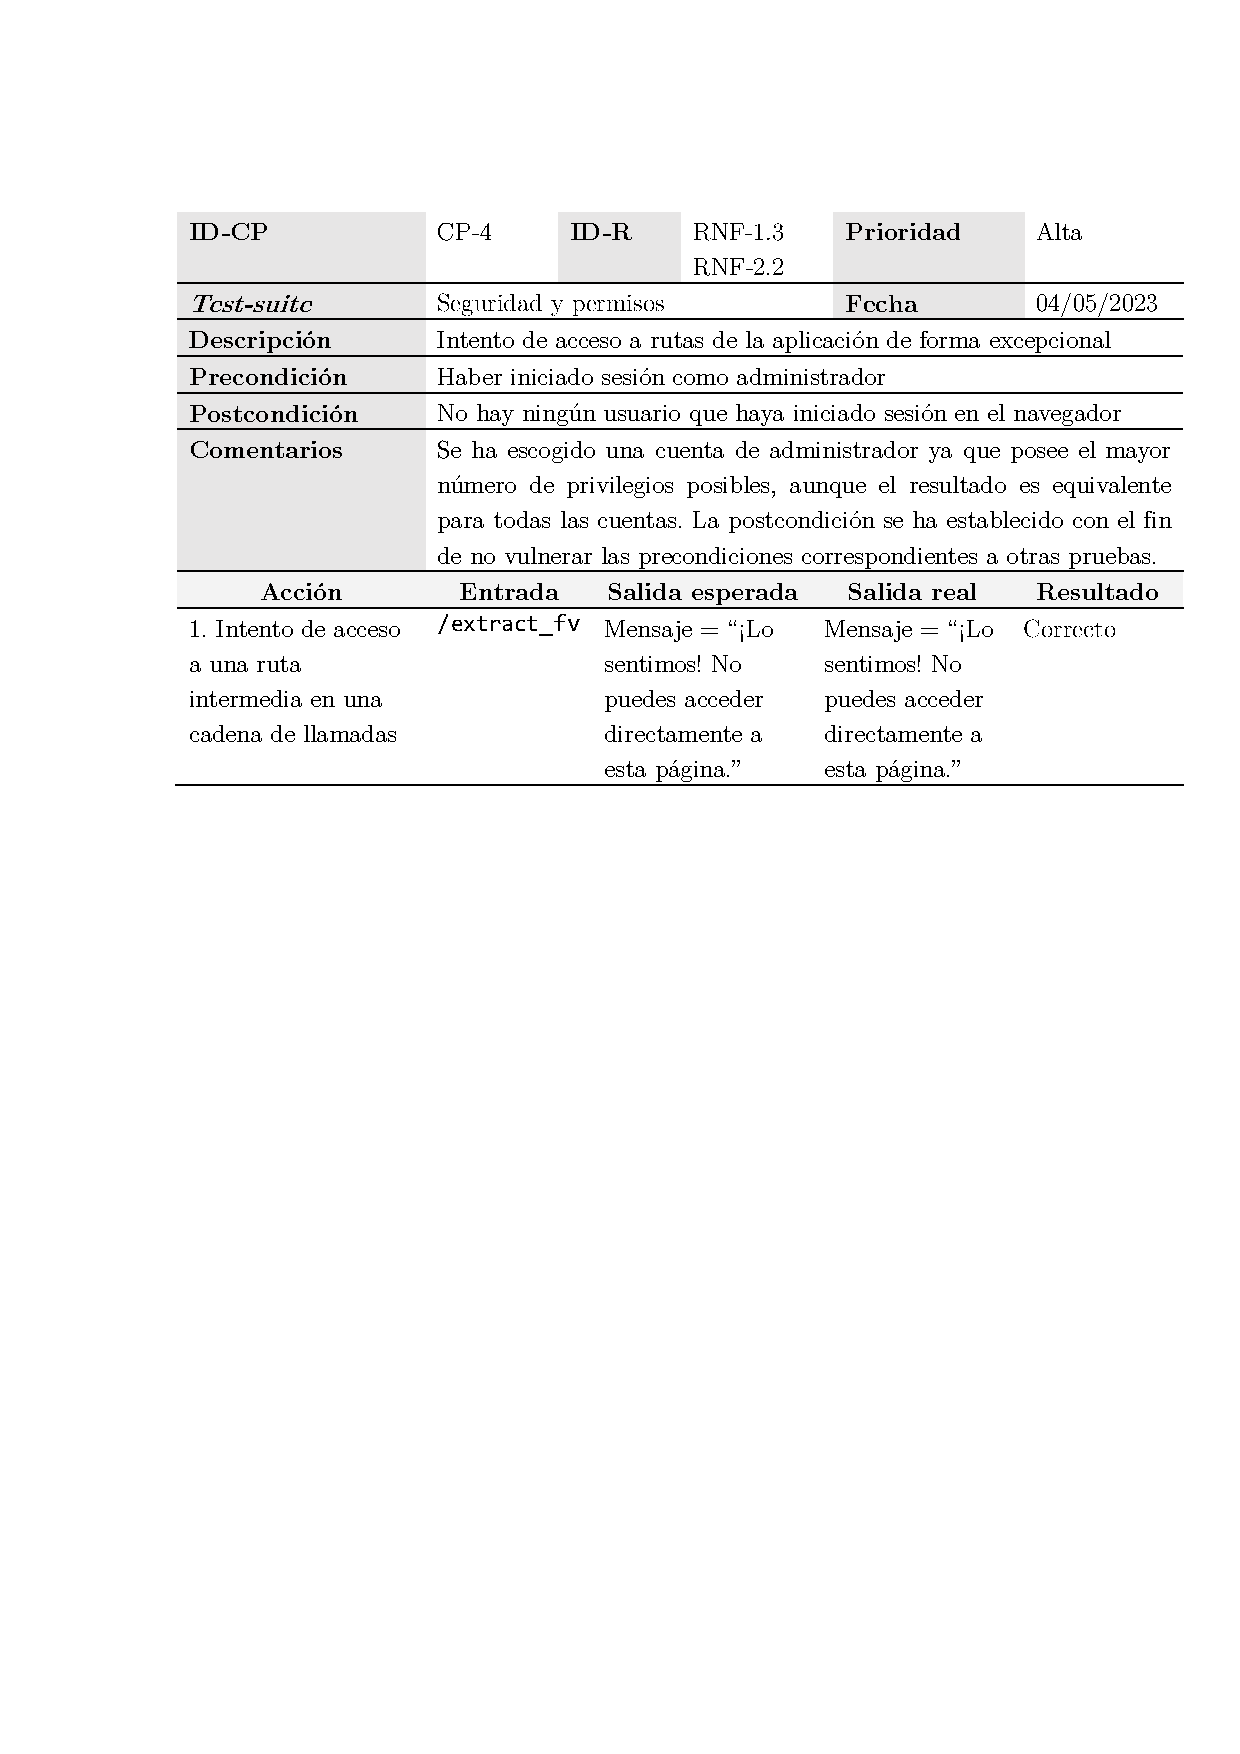
\includegraphics[width=\textwidth]{../img/anexos/cp/CP-4}
	\caption{CP-4 Acceso a rutas excepcionales.}
	\label{cp:wrong-stream}
\end{table}

\begin{table}[p]
	\centering
	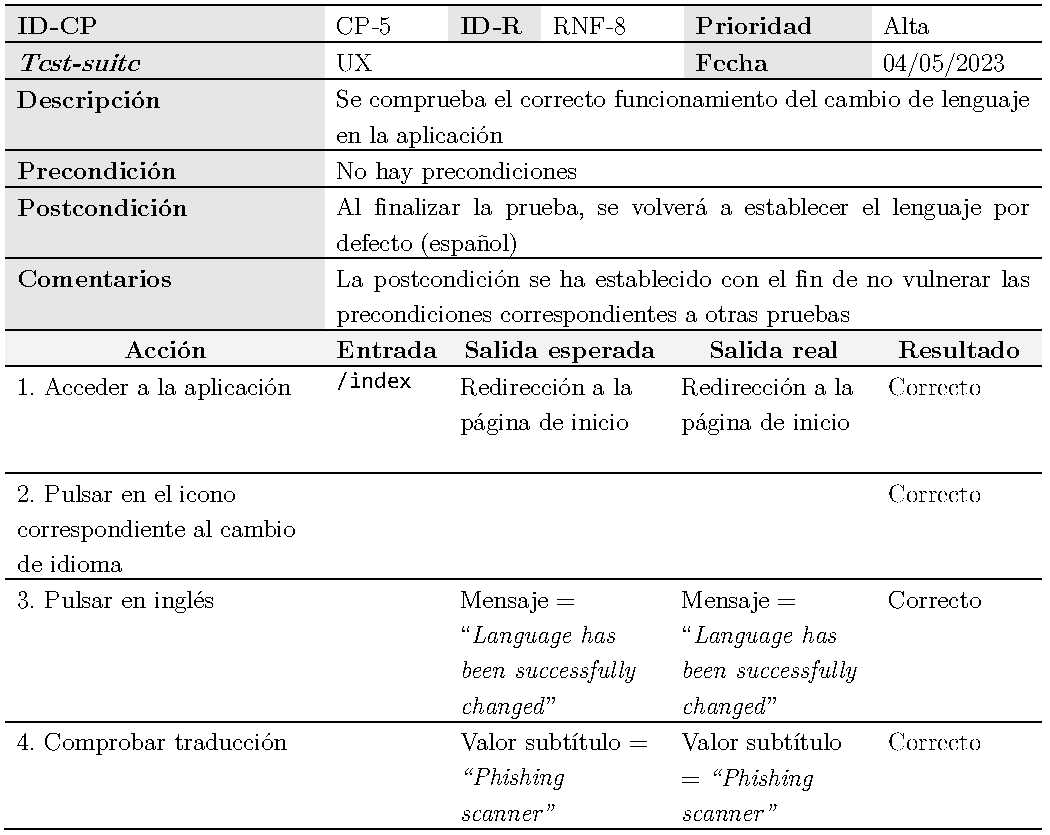
\includegraphics[width=\textwidth]{../img/anexos/cp/CP-5}
	\caption{CP-5 Cambio de lenguaje.}
	\label{cp:language}
\end{table}

\begin{table}[p]
	\centering
	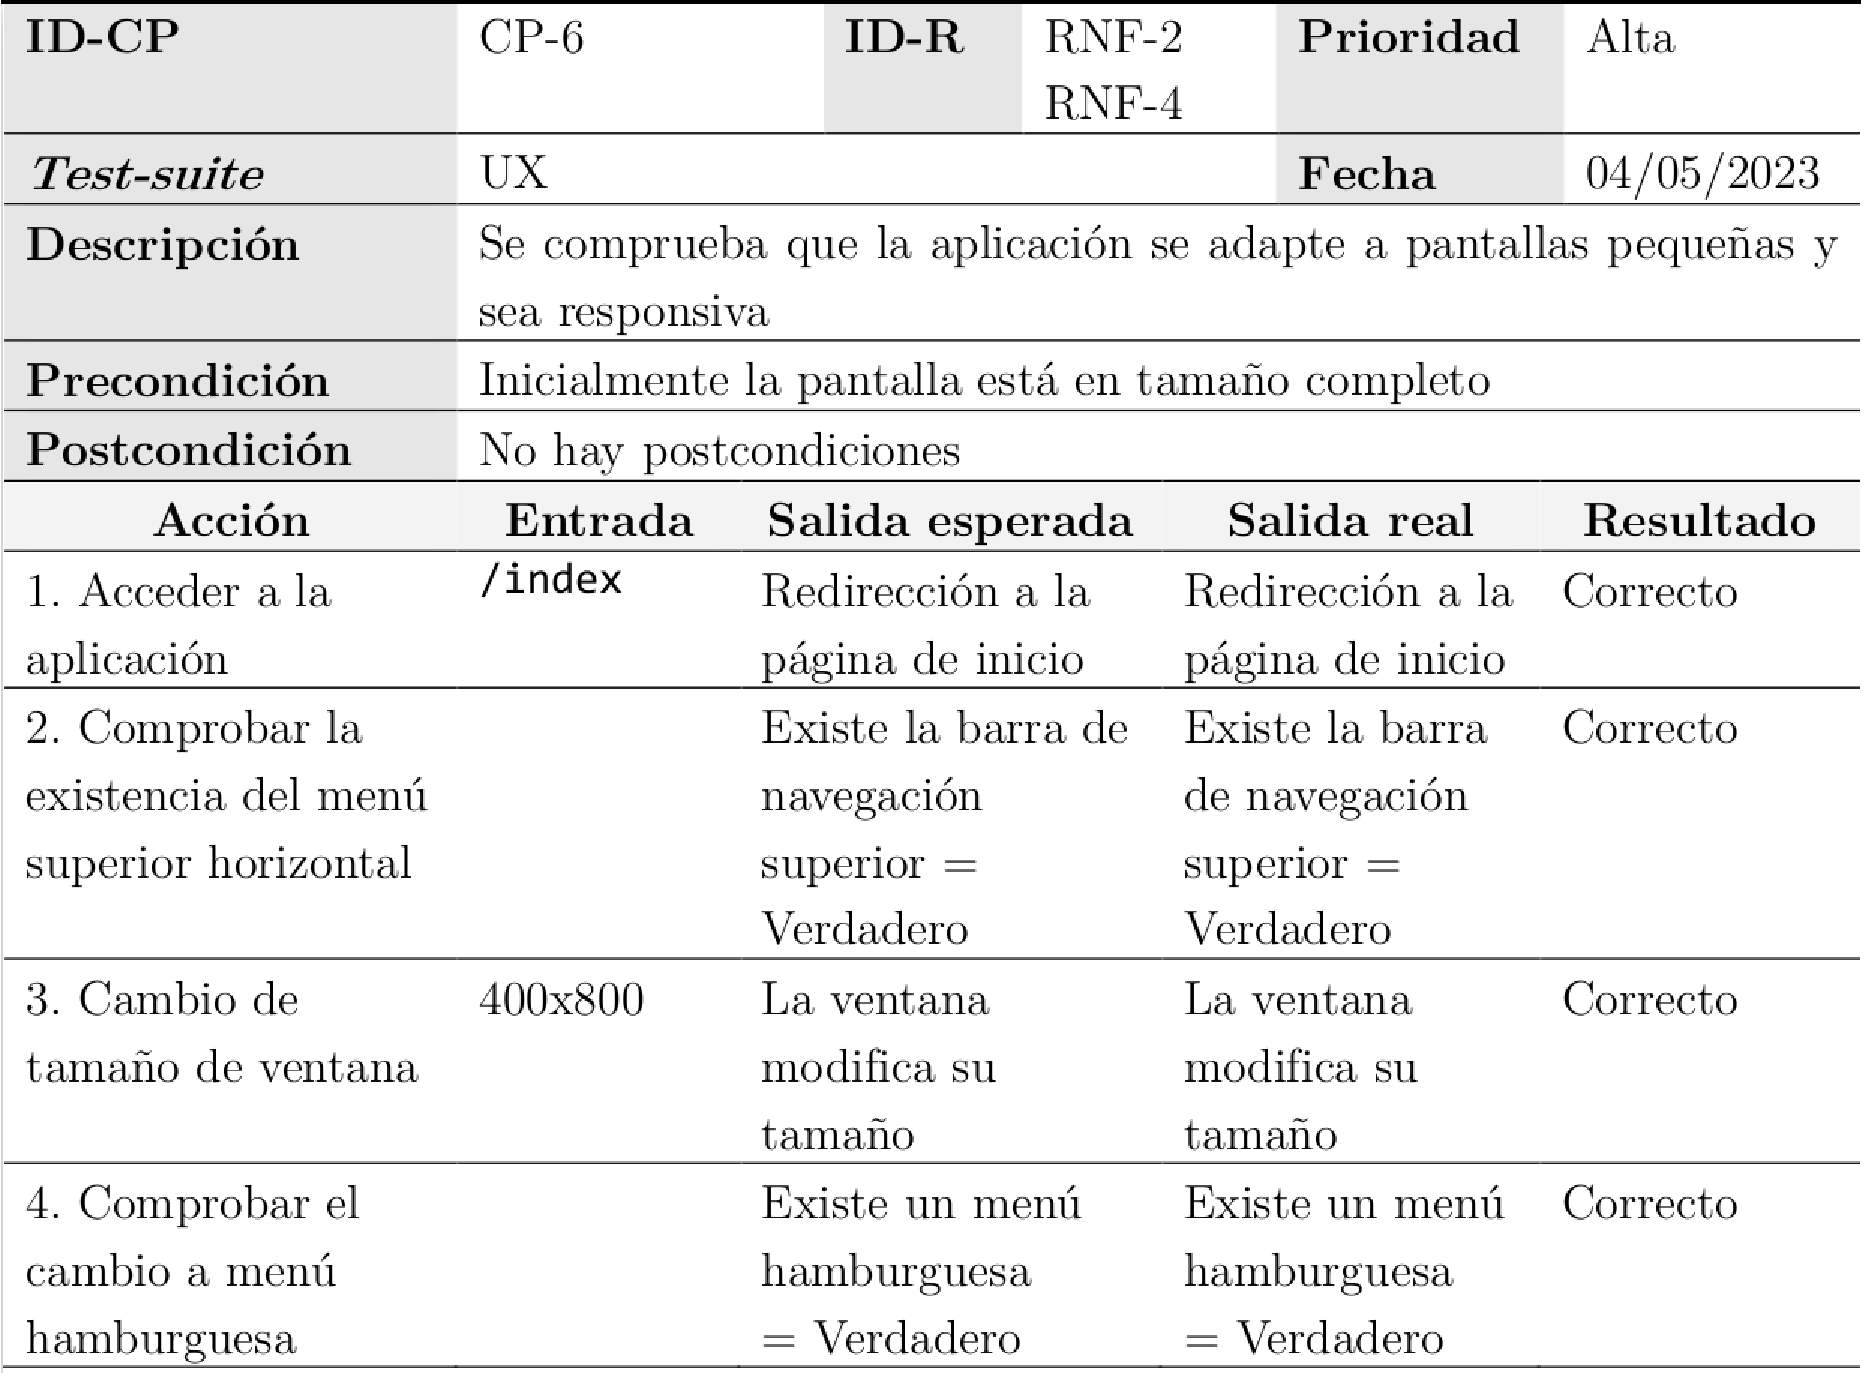
\includegraphics[width=\textwidth]{../img/anexos/cp/CP-6}
	\caption{CP-6 Pantallas responsivas.}
	\label{cp:hamburguer-menu}
\end{table}

\begin{table}[p]
	\centering
	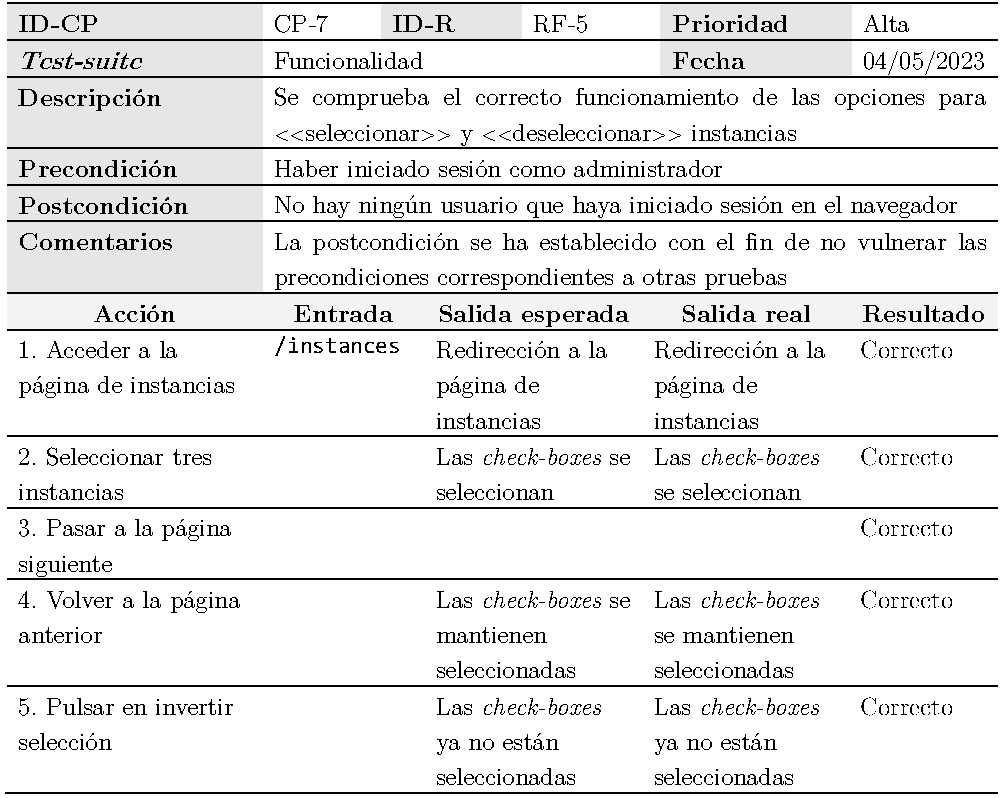
\includegraphics[width=\textwidth]{../img/anexos/cp/CP-7}
	\caption{CP-7 Funcionamiento de las \textit{check-boxes}.}
	\label{cp:checkboxes}
\end{table}

\begin{table}[p]
	\centering
	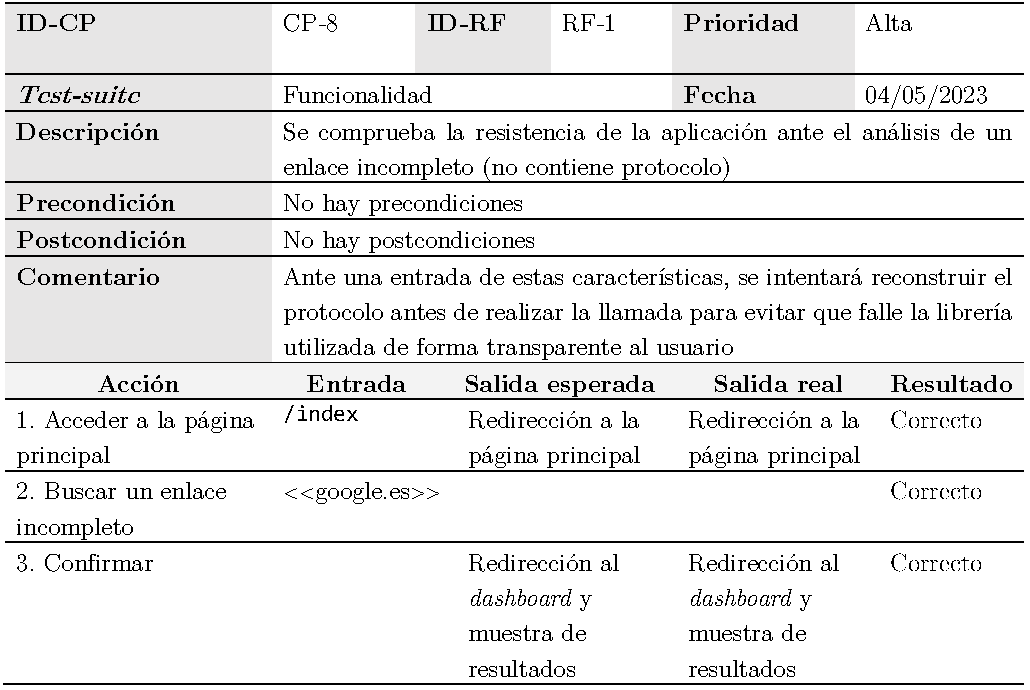
\includegraphics[width=\textwidth]{../img/anexos/cp/CP-8}
	\caption{CP-8 Análisis enlace incompleto.}
	\label{cp:url-incompleta}
\end{table}

\begin{table}[p]
	\centering
	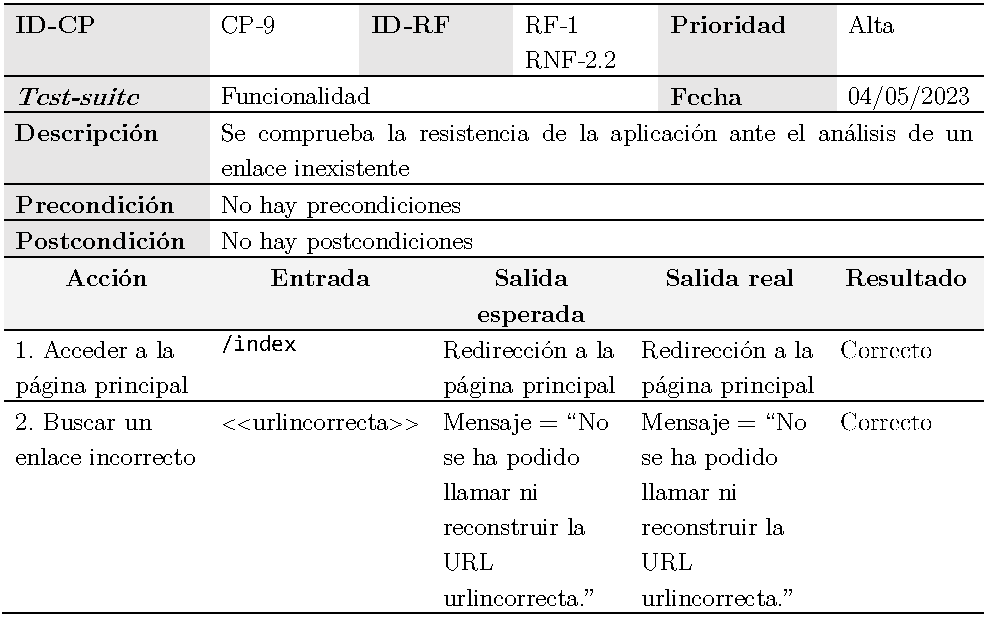
\includegraphics[width=\textwidth]{../img/anexos/cp/CP-9}
	\caption{CP-9 Análisis enlace erróneo.}
	\label{cp:wrong-url}
\end{table}

\begin{table}[p]
	\centering
	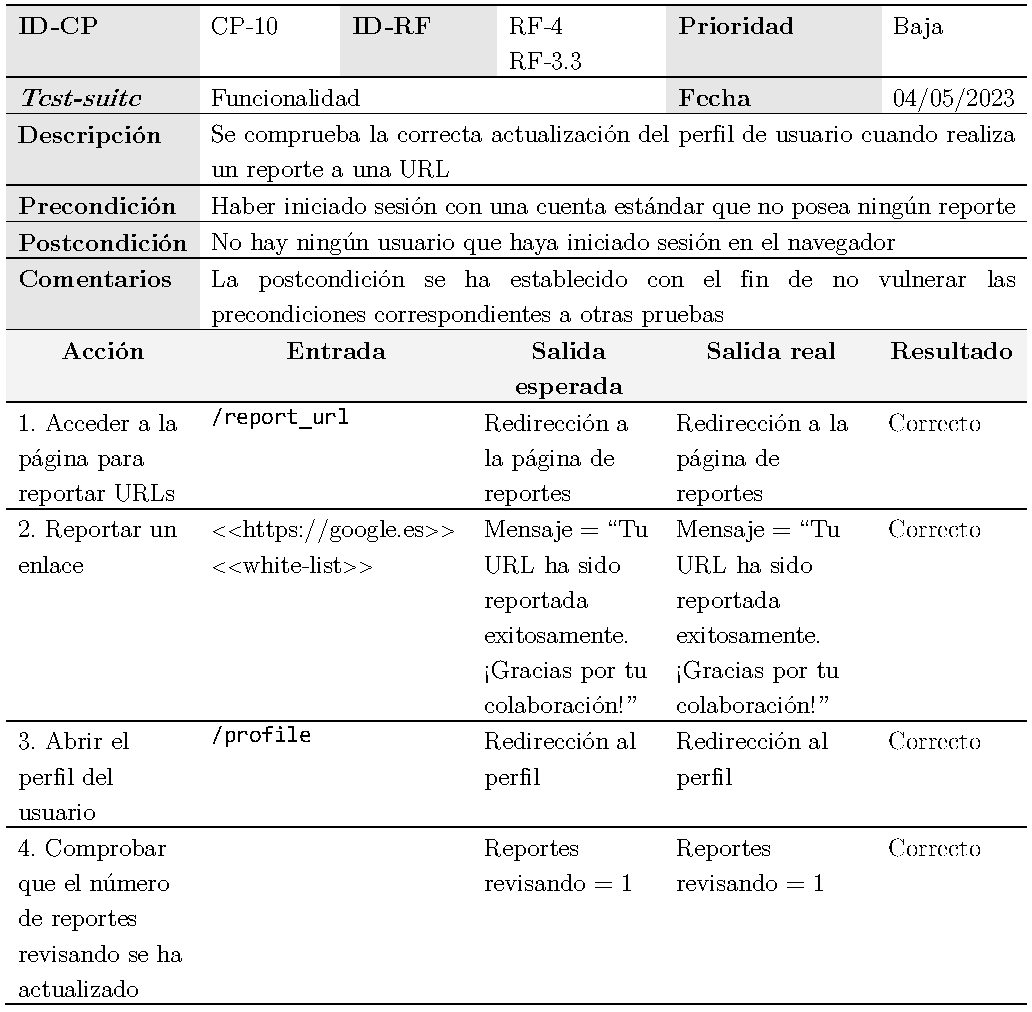
\includegraphics[width=\textwidth]{../img/anexos/cp/CP-10}
	\caption{CP-10 Actualización del perfil con las denuncias de URLs.}
	\label{cp:report-url}
\end{table}

\begin{table}[p]
	\centering
	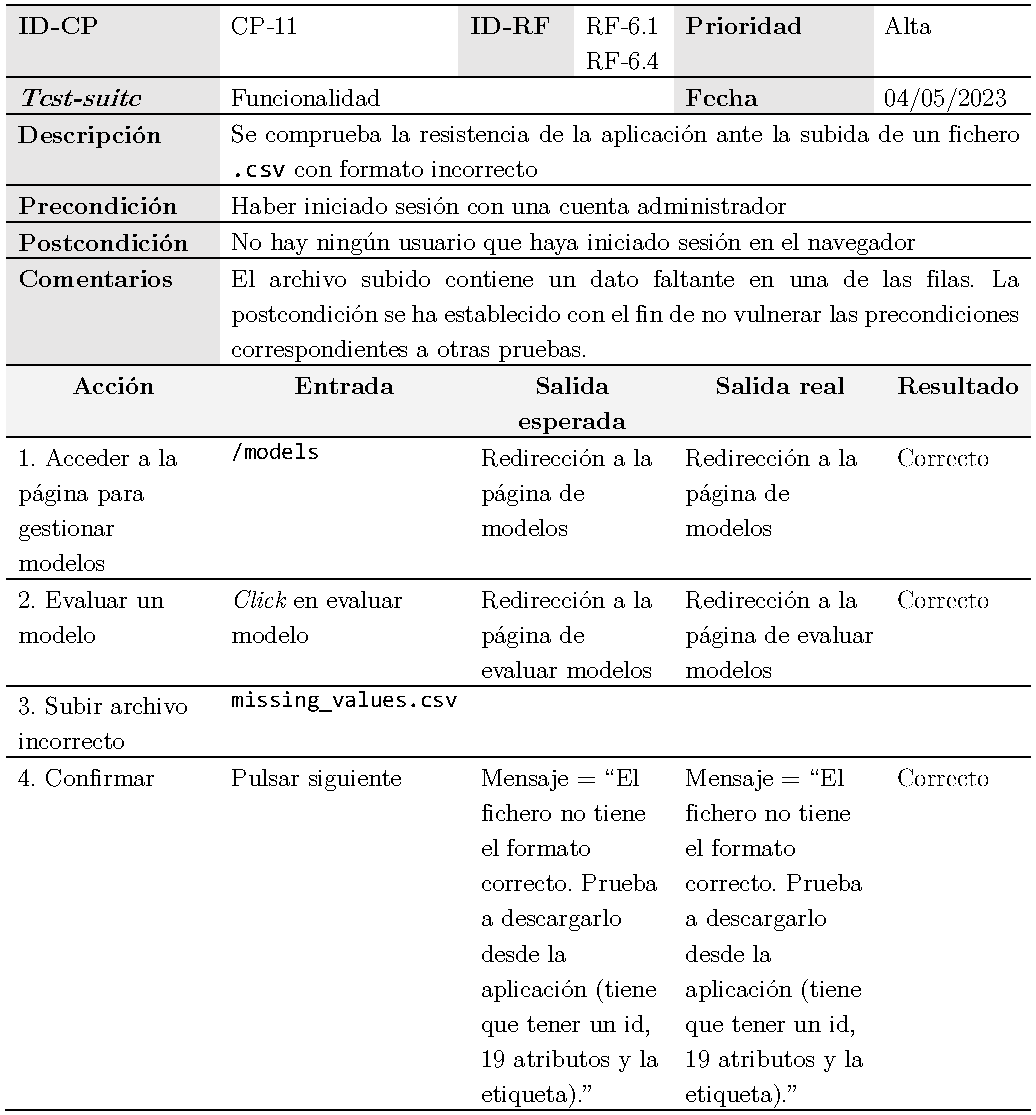
\includegraphics[width=\textwidth]{../img/anexos/cp/CP-11}
	\caption{CP-11 \texttt{csv} con formato incorrecto.}
	\label{cp:wrong-csv}
\end{table}

\begin{table}[p]
	\centering
	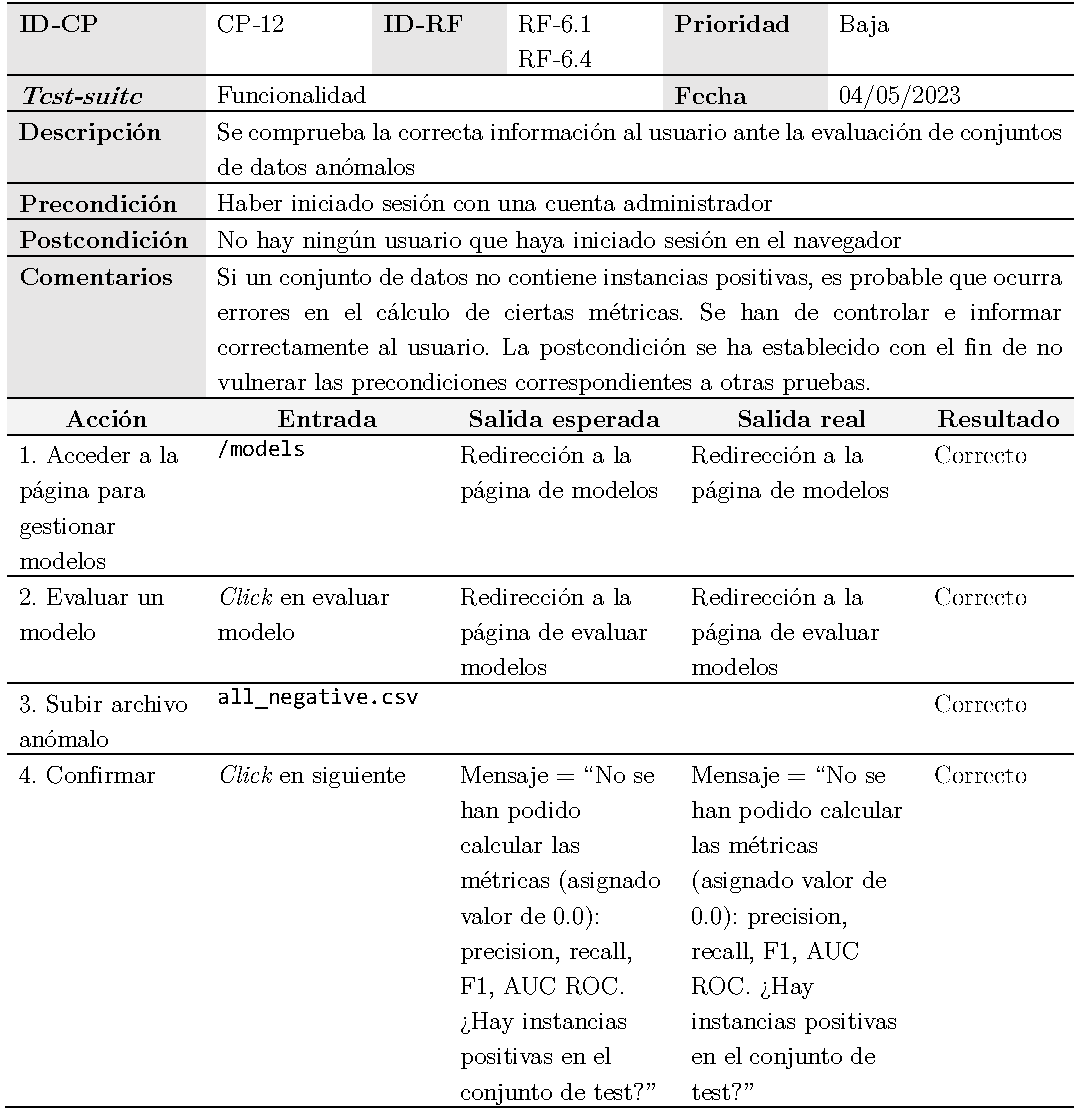
\includegraphics[width=\textwidth]{../img/anexos/cp/CP-12}
	\caption{CP-12 \texttt{csv} con conjunto de \textit{test} anómalo.}
	\label{cp:strange-csv}
\end{table}